\begin{figure}[H]
  \centering
  \pgfplotsset{
    scaled y ticks=false,
    scale only axis,
    legend style={at={(0,0.8)}, anchor=west, font=\tiny},
    xmin=7,
  }
  
  
  \begin{tikzpicture}
  \begin{groupplot}[
      group style={
          group name=my fancy plots,
          group size=1 by 2,
          xticklabels at=edge bottom,
          vertical sep=0pt
      },
  %    width=8.5cm,
      xmin=7, xmax=14
  ]
  \nextgroupplot[ymin=100000,ymax=270000,
 %                ytick={0},
                 axis x line=top,
                       axis y discontinuity=parallel, height=4.0cm
                ]
      \addplot[smooth,mark=*,mark options={solid},black]
      coordinates{ (7,256300) (8,254888) (9,144484) (10,194390) (11,135874) (12,233684) (13,243624) (14,221408)
      }; \label{int_plot} \addlegendentry{Integer}  
  \nextgroupplot[ymin=8000,ymax=30000,
%                 ytick={60,80},
  %               axis x line=top, 
                 height=15.5cm]
      \addplot[smooth,mark=square*, mark options={solid},red, dashed]
      coordinates{ (7,29788) (8,16760) (9,8770) (10,14248) (11,11456) (12,14602) (13,17456) (14,13112)
      }; \label{ie_plot} \addlegendentry{IntPairExact}
      \addplot[smooth,mark=square*, mark options={solid},blue, dotted]
      coordinates{ (7,30142) (8,16836) (9,8960) (10,14390) (11,11584) (12,14694) (13,17634) (14,13242)
      }; \label{ia_plot} \addlegendentry{IntPairApprox}
  

  \end{groupplot}
  \end{tikzpicture}
  
  
  
  
  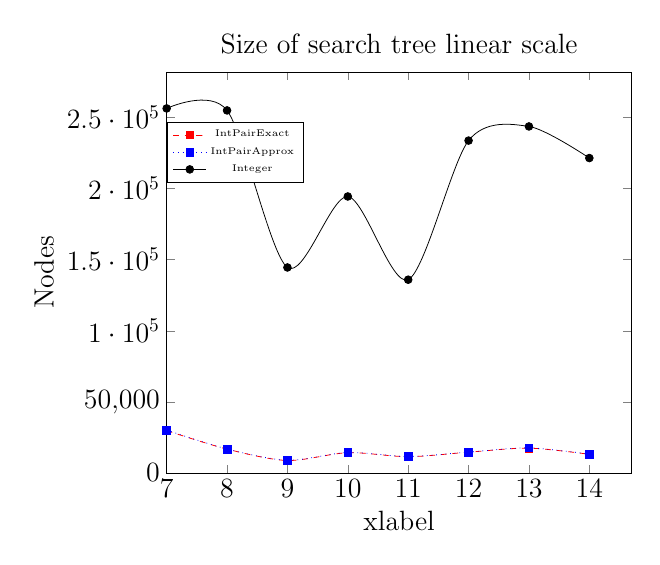
\begin{tikzpicture} [scale=0.7, font=\Large]
    \begin{axis}[
        title=Size of search tree linear scale,
        ylabel=Nodes,
        xtick=data,
        ymin=0, 
        xlabel=xlabel ]
      \addplot[smooth,mark=square*, mark options={solid},red, dashed]
      coordinates{ (7,29788) (8,16760) (9,8770) (10,14248) (11,11456) (12,14602) (13,17456) (14,13112)
      }; \label{ie_plot} \addlegendentry{IntPairExact}
      \addplot[smooth,mark=square*, mark options={solid},blue, dotted]
      coordinates{ (7,30142) (8,16836) (9,8960) (10,14390) (11,11584) (12,14694) (13,17634) (14,13242)
      }; \label{ia_plot} \addlegendentry{IntPairApprox}
      \addplot[smooth,mark=*,mark options={solid},black]
      coordinates{ (7,256300) (8,254888) (9,144484) (10,194390) (11,135874) (12,233684) (13,243624) (14,221408)
      }; \label{int_plot} \addlegendentry{Integer}
    \end{axis}
  \end{tikzpicture}
  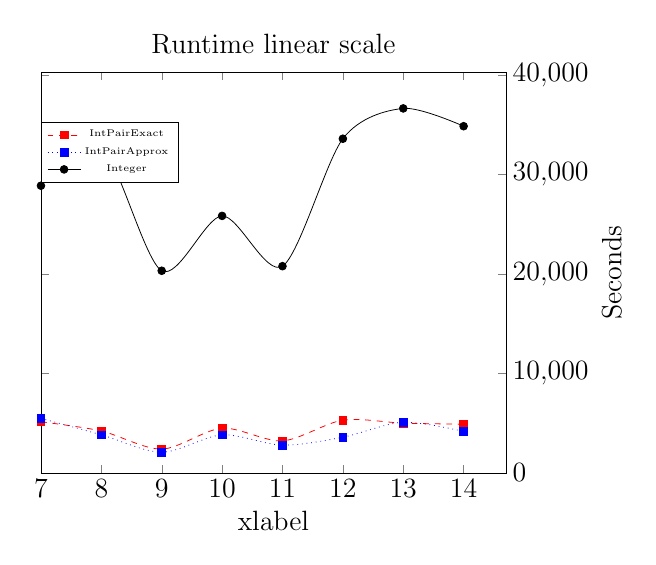
\begin{tikzpicture} [scale=0.7, font=\Large]
    \begin{axis}[
        yticklabel pos=right,
        xtick=data,
        title=Runtime linear scale,
        ylabel=Seconds,
        xlabel=xlabel,
        ymin=0, ]
      \addplot[smooth,mark=square*,mark options={solid},red, dashed]
      coordinates{ (7, 5146) (8, 4220) (9, 2397) (10, 4500) (11, 3223) (12, 5308) (13, 5009) (14, 4901)
      }; \label{IntPairExact Run}
      \addplot[smooth,mark=square*,mark options={solid},blue, dotted]
      coordinates{ (7, 5483) (8, 3837) (9, 2080) (10, 3829) (11, 2794) (12, 3593) (13, 5102) (14, 4179)
      }; \label{IntPairApprox Run}
      \addplot[smooth,mark=*,mark options={solid},black]
      coordinates{ (7, 28869) (8, 32743) (9, 20322) (10, 25837) (11, 20783) (12, 33592) (13, 36638) (14, 34850)
      }; \label{IntegerRun}
      \addlegendentry{IntPairExact}
      \addlegendentry{IntPairApprox}
      \addlegendentry{Integer}
    \end{axis}
  \end{tikzpicture}

  
\begin{tikzpicture}[scale=1.4]
    \draw[very thick] (-4,0) -- (4,0);
    \draw[draw=white] (-5,-0.2) -- (5,-0.2);
  \end{tikzpicture}


  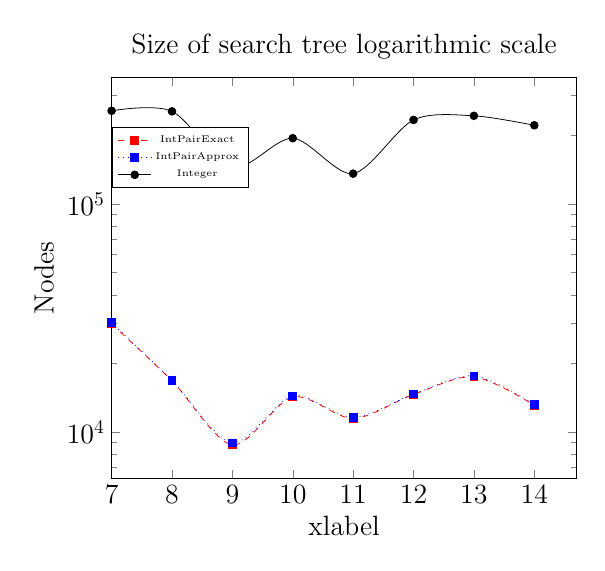
\begin{tikzpicture} [scale=0.7, font=\Large]
    \begin{semilogyaxis}[
        title=Size of search tree logarithmic scale,
        ylabel=Nodes,
        xtick=data,
        ymin=0, 
        xlabel=xlabel ]
     \addplot[smooth,mark=square*, mark options={solid},red, dashed]
      coordinates{ (7,29788) (8,16760) (9,8770) (10,14248) (11,11456) (12,14602) (13,17456) (14,13112)
      }; \label{ie_plot} \addlegendentry{IntPairExact}
      \addplot[smooth,mark=square*, mark options={solid},blue, dotted]
      coordinates{ (7,30142) (8,16836) (9,8960) (10,14390) (11,11584) (12,14694) (13,17634) (14,13242)
      }; \label{ia_plot} \addlegendentry{IntPairApprox}
      \addplot[smooth,mark=*,mark options={solid},black]
      coordinates{ (7,256300) (8,254888) (9,144484) (10,194390) (11,135874) (12,233684) (13,243624) (14,221408)
      }; \label{int_plot} \addlegendentry{Integer}

    \end{semilogyaxis}
  \end{tikzpicture}
  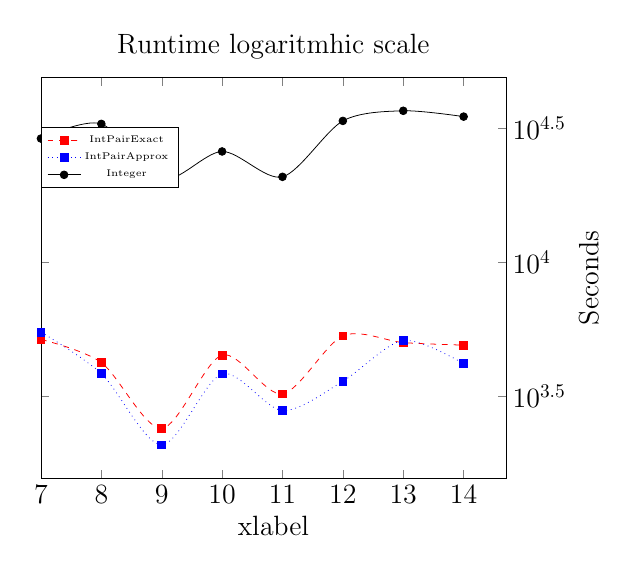
\begin{tikzpicture} [scale=0.7, font=\Large]
    \begin{semilogyaxis}[
        title=Runtime logaritmhic scale,
        yticklabel pos=right,
        xtick=data,
        ylabel=Seconds,
        xlabel=xlabel,
        ymin=0,  ]
      \addplot[smooth,mark=square*,mark options={solid},red, dashed]
      coordinates{ (7, 5146) (8, 4220) (9, 2397) (10, 4500) (11, 3223) (12, 5308) (13, 5009) (14, 4901)
      }; \label{IntPairExact Run}
      \addplot[smooth,mark=square*,mark options={solid},blue, dotted]
      coordinates{ (7, 5483) (8, 3837) (9, 2080) (10, 3829) (11, 2794) (12, 3593) (13, 5102) (14, 4179)
      }; \label{IntPairApprox Run}
      \addplot[smooth,mark=*,mark options={solid},black]
      coordinates{ (7, 28869) (8, 32743) (9, 20322) (10, 25837) (11, 20783) (12, 33592) (13, 36638) (14, 34850)
      }; \label{IntegerRun}
      \addlegendentry{IntPairExact}
      \addlegendentry{IntPairApprox}
      \addlegendentry{Integer}
    \end{semilogyaxis}
  \end{tikzpicture}
  \caption{Varying the number of states. The other parameters are fixed: $symbols=10$, $cost=20$, and $steps=7$.}\label{fig:states}
\end{figure}
